
\documentclass[11pt,a4paper]{article}

% ---------------------------------------------
% Packages
% ---------------------------------------------
\usepackage[utf8]{inputenc}
\usepackage[T1]{fontenc}
\usepackage{lmodern}
\usepackage{microtype}
\usepackage{geometry}
\geometry{margin=1in}

\usepackage{amsmath,amssymb,amsfonts,amsthm,mathtools}
\usepackage{bm}
\usepackage{bbm}

\usepackage{graphicx}
\usepackage{booktabs}
\usepackage{caption}
\usepackage{subcaption}

\usepackage{algorithm}
\usepackage{algpseudocode}

\usepackage{xcolor}
\usepackage{soul} % Added for highligting
\usepackage{hyperref}
\hypersetup{
  colorlinks=true,
  linkcolor=blue,
  citecolor=blue,
  urlcolor=blue
}

\usepackage{fancyhdr}
\usepackage{tikz}
\usetikzlibrary{positioning,arrows.meta,shapes.geometric,fit,calc,backgrounds,decorations.pathreplacing}

% ---------------------------------------------
% Header / Footer
% ---------------------------------------------
\pagestyle{fancy}
\fancyhf{}
\lhead{Research Draft}
\rhead{Physics-Informed Map-Conditioned UE Localization}
\cfoot{\thepage}
\setlength{\headheight}{14pt}

% ---------------------------------------------
% Macros
% ---------------------------------------------
\newcommand{\R}{\mathbb{R}}
\newcommand{\E}{\mathbb{E}}
\newcommand{\Var}{\mathrm{Var}}
\newcommand{\Cov}{\mathrm{Cov}}
\newcommand{\KL}{\mathrm{KL}}
\newcommand{\softmax}{\mathrm{softmax}}
\newcommand{\diag}{\mathrm{diag}}
\newcommand{\tr}{\mathrm{tr}}
\DeclareMathOperator*{\argmax}{arg\,max}
\DeclareMathOperator*{\argmin}{arg\,min}
\DeclareMathOperator{\LogSumExp}{LogSumExp}

% Semantic highlighting commands
% Pink: Problems, Challenges, Constraints
\DeclareRobustCommand{\hlprob}[1]{{\sethlcolor{pink}\hl{#1}}}
% Yellow: Solutions, Key Innovations, Core Concepts
\DeclareRobustCommand{\hlsol}[1]{{\sethlcolor{yellow}\hl{#1}}}

% Theorem environments (kept lightweight; we use them for invariance statements)
\newtheorem{proposition}{Proposition}

% ---------------------------------------------
\title{\vspace{-0.8cm}\textbf{Physics-Informed Map-Conditioned Transformers for Probabilistic UE Localization}\\
\vspace{0.1cm}\large Coarse-to-Fine Mixture Posteriors, Differentiable Radio-Map Likelihoods, and Test-Time Refinement}
\author{Nir Tzur}
\date{\vspace{-0.2cm}\today}

\begin{document}
\maketitle
\vspace{-0.6cm}

\begin{abstract}
Localizing user equipment (UE) from sparse, irregular radio measurements is an \hlprob{ill-posed inverse problem}: multiple spatial hypotheses can explain the same measurements, and \hlprob{purely data-driven predictors can violate basic propagation constraints}. We present a \hlsol{map-conditioned Transformer} that amortizes Bayesian inference over UE position while remaining tightly coupled to a physics simulator through a \hlsol{differentiable radio-map likelihood}.
The model (i) encodes measurement sequences as sets of timestamped, multi-layer features, (ii) encodes multi-channel environmental context (radio maps and semantic GIS layers) via a vision Transformer, (iii) fuses both modalities with cross-attention, and (iv) outputs a \hlsol{coarse-to-fine} \hlsol{top-$K$ Gaussian mixture posterior} over 2D position.
Training combines a proper probabilistic objective (coarse cell cross-entropy + \hlsol{mixture negative log-likelihood}) with a \hlsol{physics-consistency term} computed by \hlsol{differentiable bilinear sampling} of precomputed radio maps.
At inference, the learned posterior provides calibrated uncertainty and supports optional \hlsol{MAP refinement} by gradient descent on an energy combining the network density and the physics likelihood.
We detail the model end-to-end from first principles, including the induced invariances, the probabilistic semantics of the heads, and the differentiable physics coupling.
\end{abstract}

% ---------------------------------------------
\begin{figure}[t]
\centering
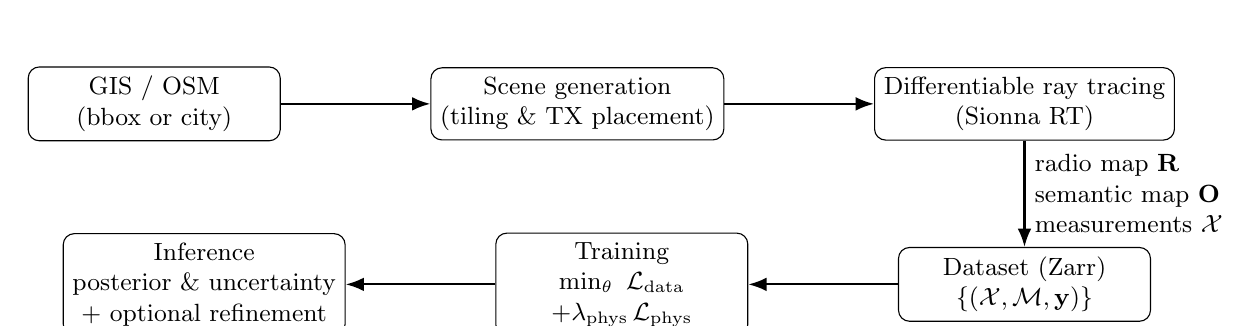
\begin{tikzpicture}[
  node distance=1.15cm,
  >=Latex,
  font=\small,
  block/.style={draw, rounded corners, align=center, minimum width=3.2cm, minimum height=0.9cm},
  arrow/.style={->, thick}
]
\node[block] (gis) {GIS / OSM\\(bbox or city)};
\node[block, right=1.9cm of gis] (scene) {Scene generation\\(tiling \& TX placement)};
\node[block, right=1.9cm of scene] (rt) {Differentiable ray tracing\\(Sionna RT)};
\node[block, below=1.35cm of rt] (data) {Dataset (Zarr)\\$\{(\mathcal{X},\mathcal{M},\mathbf{y})\}$};
\node[block, left=1.9cm of data] (train) {Training\\$\min_\theta~\mathcal{L}_{\text{data}}$\\$+\lambda_{\text{phys}}\,\mathcal{L}_{\text{phys}}$};
\node[block, left=1.9cm of train] (infer) {Inference\\posterior \& uncertainty\\+ optional refinement};

\draw[arrow] (gis) -- (scene);
\draw[arrow] (scene) -- (rt);
\draw[arrow] (rt) -- node[right, align=left] {radio map $\mathbf{R}$\\semantic map $\mathbf{O}$\\measurements $\mathcal{X}$} (data);
\draw[arrow] (data) -- (train);
\draw[arrow] (train) -- (infer);
\end{tikzpicture}
\vspace{-0.2cm}
\caption{End-to-end pipeline: GIS/OSM $\rightarrow$ scenes and deployments $\rightarrow$ differentiable RT $\rightarrow$ dataset $\rightarrow$ training $\rightarrow$ probabilistic inference with optional refinement.}
\label{fig:pipeline}
\end{figure}

% ---------------------------------------------
\section{Introduction}

UE localization from sparse radio measurements under complex urban propagation is central to digital twins, network planning, and context-aware communications. Yet it poses two fundamental difficulties.

First, the inverse map from measurements to position is \hlprob{multi-valued}: different locations can generate similar received power/quality patterns due to shadowing, multipath, and limited sampling.
Second, the forward physics is constrained (e.g., occlusion by buildings, diffraction/reflection structure), and \hlprob{purely data-driven regressors can produce predictions that are not physically plausible}.

This work treats localization as \hlsol{probabilistic inference} with explicit environmental conditioning. We assume access to a multi-channel map context $\mathcal{M}$ (semantic GIS layers and/or precomputed radio fields) and a variable-length measurement sequence $\mathcal{X}$. We learn an amortized posterior $p_\theta(\mathbf{y}\mid \mathcal{X},\mathcal{M})$ over UE position $\mathbf{y}\in\R^2$.
To capture multi-modality at scale, we represent the posterior as a \hlsol{coarse-to-fine} \hlsol{top-$K$ Gaussian mixture} tied to a coarse spatial grid.
To enforce physics consistency, we add a \hlsol{differentiable radio-map likelihood term}: predicted positions must align with precomputed radio-map features when sampled via bilinear interpolation.
Finally, we expose a principled refinement mechanism: when needed, we optimize a \hlsol{MAP objective} combining the learned posterior and the physics likelihood.

\paragraph{Contributions.}
\begin{itemize}
\item \hlsol{Map-conditioned Transformer posterior.} A dual-encoder architecture (Transformer-based radio encoder with \texttt{[CLS]} pooling + map ViT with optional E(2)-equivariance) fused by multi-query cross-attention.
\item \hlsol{Coarse-to-fine mixture density head.} A hierarchical discretize-then-refine posterior $p(\mathbf{y})=\sum_c \pi_c\,\mathcal{N}(\mathbf{y};\bm\mu_c,\bm\Sigma_c)$ with a top-$K$ truncation that preserves multi-modality while controlling compute.
\item \hlsol{Differentiable physics coupling.} A physics-consistency loss derived as a negative log-likelihood under a measurement noise model, computed via \hlsol{differentiable sampling} of precomputed radio fields.
\item \hlsol{MAP refinement.} An inference-time energy minimization that improves low-confidence predictions while remaining consistent with the learned posterior.
\end{itemize}

% ---------------------------------------------
\section{Related Work}

\textbf{Differentiable radio propagation.}
Differentiable ray tracing enables gradients of propagation quantities with respect to scene and system parameters, supporting inverse problems and end-to-end optimization. Sionna RT provides a differentiable ray tracer for radio propagation modeling and radio-map computation \cite{hoydis2023sionnart,aitaoudia2025sionna_techreport}. RayLoc reformulates localization as an inverse ray-tracing problem with fully differentiable simulation \cite{han2025rayloc}. Unlike fully differentiable localization pipelines that invoke ray tracing during inference, we amortize inference with a neural posterior conditioned on precomputed maps, and optionally apply local physics refinement when needed. WiNeRT explores neural surrogates for wireless ray tracing, aiming for fast differentiable signal rendering \cite{orekondy2023winert}.

\textbf{Radio map estimation and learning with maps.}
CNN-based estimators such as RadioUNet learn to predict pathloss/radio maps from urban context \cite{levie2021radiounet}. Transformer-based estimators have recently shown strong performance and favorable inductive biases for sparse spatial observations; STORM is an attention-based estimator for radio map estimation and active sensing \cite{viet2024storm}, and TransPathNet combines transformer feature extraction with multiscale decoding for indoor pathloss mapping \cite{li2025transpathnet}. Physics-informed neural networks have also been proposed for radio environment mapping by embedding PDE residuals as soft constraints \cite{shahid2025reveal,shahid2025revealmt}.

\textbf{Set-structured and probabilistic prediction.}
Measurement sequences are irregular and naturally set-valued; Deep Sets characterizes permutation-invariant set functions \cite{zaheer2017deepsets}, and Set Transformer provides an attention-based framework for permutation-invariant/equivariant learning on sets \cite{lee2019settransformer}. For multi-modal regression, mixture density networks (MDNs) parameterize conditional densities via mixtures \cite{bishop1994mdn}. Our method combines these ideas: set-structured radio encoding, map-conditioned attention, and a mixture posterior with an explicit physics likelihood term.

% ---------------------------------------------
\section{Problem Formulation from First Principles}
\label{sec:problem}

\subsection{Forward model and inverse objective}

Let $\mathcal{E}$ denote the environment (geometry, materials, terrain) and $\mathcal{T}$ the transmitter deployment (sites, antenna patterns, carrier frequency, bandwidth, etc.). For a UE location $\mathbf{y}\in\R^2$ (2D ground plane for simplicity), a physics simulator induces a \emph{forward operator}
\begin{equation}
  \Phi_{\mathcal{E},\mathcal{T}}:\R^2 \rightarrow \R^{C_r}, 
  \qquad \mathbf{r}(\mathbf{y}) = \Phi_{\mathcal{E},\mathcal{T}}(\mathbf{y}),
\end{equation}
where $\mathbf{r}(\mathbf{y})$ is a vector of radio features (e.g., path gain, SNR, SINR, throughput, BLER, ToA/AoA when available). In practice, we precompute $\Phi_{\mathcal{E},\mathcal{T}}$ on a grid to obtain a \emph{radio map} $\mathbf{R}\in\R^{C_r\times H\times W}$ and sample it continuously at arbitrary $\mathbf{y}$ via differentiable interpolation (Sec.~\ref{sec:lookup}).

We observe a sparse sequence of measurement events $\mathcal{X}$ collected over time and potentially across cells/beams. Abstractly, for each event $t\in\{1,\dots,T\}$,
\begin{equation}
  \mathbf{x}_t = (\underbrace{c_t,b_t}_{\text{IDs}},~\underbrace{\tau_t}_{\text{time}},~\underbrace{\mathbf{f}_t}_{\text{features}}),
  \qquad \mathbf{f}_t \in \R^{d},
\end{equation}
where $c_t$ and $b_t$ denote categorical identifiers (cell/beam) and $\mathbf{f}_t$ concatenates multi-layer features (ray-tracing statistics, PHY metrics, MAC metrics, etc.). The inverse goal is to infer $\mathbf{y}$ given $\mathcal{X}$ and map context $\mathcal{M}$:
\begin{equation}
  \text{infer } \mathbf{y}\quad \text{from}\quad (\mathcal{X},\mathcal{M}),
\end{equation}
where $\mathcal{M}$ may include a semantic map $\mathbf{O}\in\R^{C_o\times H\times W}$ and the radio map $\mathbf{R}$ (or a subset of channels). 

A principled approach is Bayesian inference with a posterior $p(\mathbf{y}\mid \mathcal{X},\mathcal{M})$. We learn an amortized approximation $p_\theta(\mathbf{y}\mid \mathcal{X},\mathcal{M})$ with explicit uncertainty.

\subsection{Coordinate system and discretization}

Let the physical extent be the rectangle $\Omega=[x_{\min},x_{\max}]\times[y_{\min},y_{\max}]$ in meters. We discretize $\Omega$ into a $G\times G$ grid of cells $\{\Omega_c\}_{c=1}^{G^2}$ with cell size $s_x=(x_{\max}-x_{\min})/G$ and $s_y=(y_{\max}-y_{\min})/G$.
Let $\mathbf{c}_c\in\R^2$ be the center of cell $\Omega_c$.
Define the cell-index function $c(\mathbf{y})$ as the unique index such that $\mathbf{y}\in\Omega_{c(\mathbf{y})}$, and denote its center by $\mathbf{c}(\mathbf{y})\triangleq\mathbf{c}_{c(\mathbf{y})}$.
We will use a latent cell variable $C\in\{1,\dots,G^2\}$ to build a hierarchical mixture posterior (Sec.~\ref{sec:posterior}).

% ---------------------------------------------
\begin{figure*}[t]
\centering
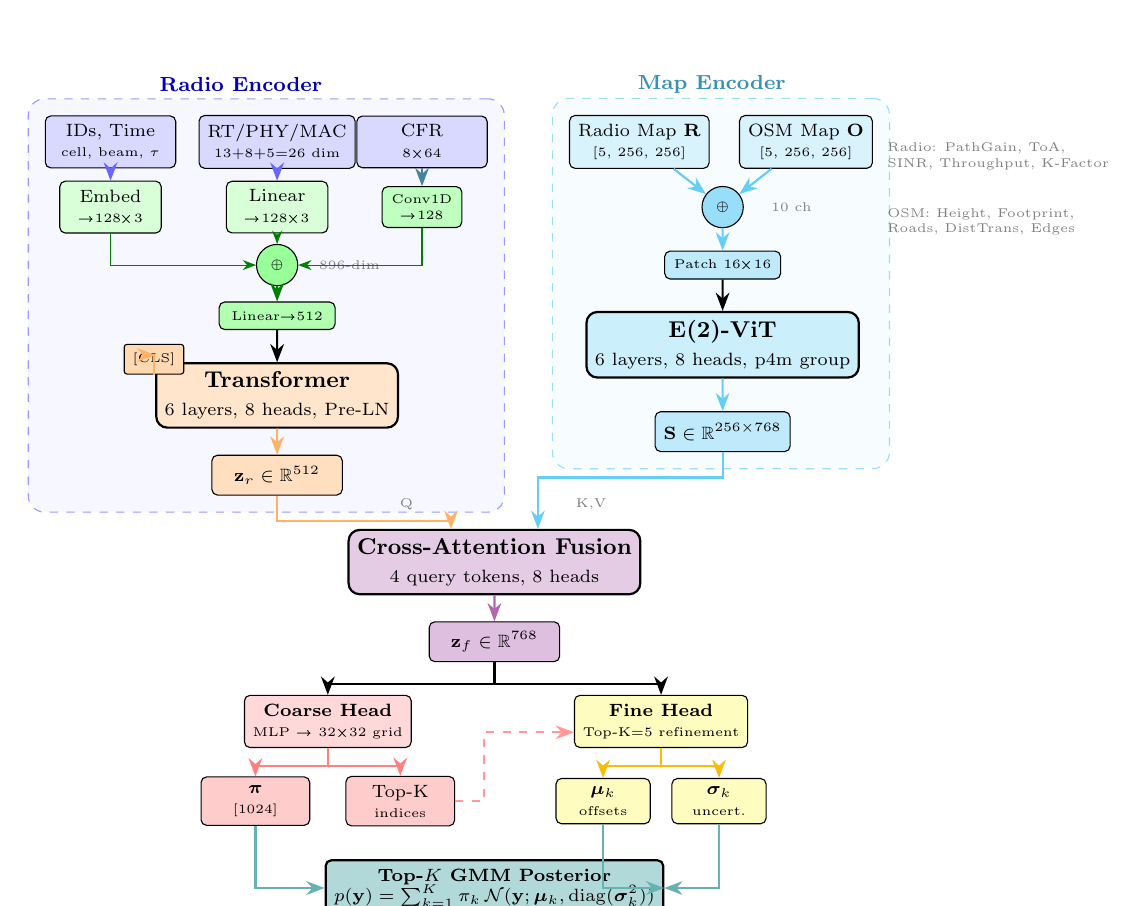
\begin{tikzpicture}[
    node distance=0.5cm and 0.7cm,
    >=Latex,
    font=\small,
    scale=0.92,
    transform shape,
    % Block styles with colors
    inputbox/.style={draw, rounded corners=2pt, fill=blue!15, minimum width=1.8cm, minimum height=0.55cm, align=center},
    embedbox/.style={draw, rounded corners=2pt, fill=green!15, minimum width=1.4cm, minimum height=0.45cm, align=center, font=\scriptsize},
    projbox/.style={draw, rounded corners=2pt, fill=green!25, minimum width=1.1cm, minimum height=0.38cm, align=center, font=\tiny},
    transformer/.style={draw, rounded corners=4pt, fill=orange!20, minimum width=2.8cm, minimum height=0.8cm, align=center, thick},
    fusionbox/.style={draw, rounded corners=4pt, fill=violet!20, minimum width=3.0cm, minimum height=0.7cm, align=center, thick},
    headbox/.style={draw, rounded corners=2pt, fill=red!15, minimum width=2.2cm, minimum height=0.6cm, align=center},
    outputbox/.style={draw, rounded corners=2pt, fill=teal!20, minimum width=1.8cm, minimum height=0.55cm, align=center},
    mapbox/.style={draw, rounded corners=2pt, fill=cyan!15, minimum width=1.8cm, minimum height=0.55cm, align=center},
    arrow/.style={->, thick, >=Stealth},
    dasharrow/.style={->, thick, >=Stealth, dashed},
    catarrow/.style={->, >=Stealth, green!50!black},
    dimtext/.style={font=\tiny, text=gray},
]

% ============================================
% RADIO ENCODER (Left)
% ============================================
\node[font=\footnotesize\bfseries, blue!70!black] at (-3.0, 5.3) {Radio Encoder};

% Input features
\node[inputbox, font=\scriptsize] (embin) at (-4.8, 4.5) {IDs, Time\\{\tiny cell, beam, $\tau$}};
\node[inputbox, font=\scriptsize] (featsin) at (-2.5, 4.5) {RT/PHY/MAC\\{\tiny 13+8+5=26 dim}};
\node[inputbox, font=\scriptsize] (cfrin) at (-0.5, 4.5) {CFR\\{\tiny 8×64}};

% Embeddings
\node[embedbox] (embproj) at (-4.8, 3.6) {Embed\\{\tiny →128×3}};
\node[embedbox] (featproj) at (-2.5, 3.6) {Linear\\{\tiny →128×3}};
\node[projbox] (cfrproj) at (-0.5, 3.6) {Conv1D\\{\tiny →128}};

\draw[arrow, blue!60] (embin) -- (embproj);
\draw[arrow, blue!60] (featsin) -- (featproj);
\draw[arrow, cyan!60!black] (cfrin) -- (cfrproj);

% Concatenation
\node[draw, circle, fill=green!40, minimum size=0.4cm, font=\tiny\bfseries] (concat) at (-2.5, 2.8) {$\oplus$};
\node[dimtext] at (-1.5, 2.8) {896-dim};

\draw[catarrow] (embproj.south) |- (concat);
\draw[catarrow] (featproj.south) -- (concat);
\draw[catarrow] (cfrproj.south) |- (concat);

% Projection
\node[projbox, minimum width=1.6cm, fill=green!30] (inputproj) at (-2.5, 2.1) {Linear→512};
\draw[arrow, green!50!black] (concat) -- (inputproj);

% Transformer
\node[transformer] (radioenc) at (-2.5, 1.0) {\textbf{Transformer}\\{\scriptsize 6 layers, 8 heads, Pre-LN}};
\draw[arrow] (inputproj) -- (radioenc);

% CLS token
\node[draw, rounded corners=1pt, fill=orange!30, font=\tiny, minimum width=0.6cm, minimum height=0.3cm] (cls) at (-4.2, 1.5) {[CLS]};
\draw[arrow, orange!60] (cls.south) |- ([yshift=0.1cm]radioenc.north west);

% Output
\node[outputbox, fill=orange!25, font=\scriptsize] (radiocls) at (-2.5, -0.1) {$\mathbf{z}_r \in \mathbb{R}^{512}$};
\draw[arrow, orange!60] (radioenc) -- (radiocls);

% ============================================
% MAP ENCODER (Right)
% ============================================
\node[font=\footnotesize\bfseries, cyan!70!black] at (3.5, 5.3) {Map Encoder};

% Map inputs
\node[mapbox, font=\scriptsize] (radiomap) at (2.5, 4.5) {Radio Map $\mathbf{R}$\\{\tiny [5, 256, 256]}};
\node[mapbox, font=\scriptsize] (osmmap) at (4.8, 4.5) {OSM Map $\mathbf{O}$\\{\tiny [5, 256, 256]}};

% Concat
\node[draw, circle, fill=cyan!40, minimum size=0.4cm, font=\tiny\bfseries] (mapconcat) at (3.65, 3.6) {$\oplus$};
\node[dimtext] at (4.6, 3.6) {10 ch};
\draw[arrow, cyan!60] (radiomap) -- (mapconcat);
\draw[arrow, cyan!60] (osmmap) -- (mapconcat);

% Patch embed
\node[projbox, minimum width=1.6cm, fill=cyan!25] (patchemb) at (3.65, 2.8) {Patch 16×16};
\draw[arrow, cyan!60] (mapconcat) -- (patchemb);

% ViT
\node[transformer, fill=cyan!20] (mapvit) at (3.65, 1.7) {\textbf{E(2)-ViT}\\{\scriptsize 6 layers, 8 heads, p4m group}};
\draw[arrow] (patchemb) -- (mapvit);

% Spatial tokens output
\node[outputbox, fill=cyan!25, font=\scriptsize] (maptokens) at (3.65, 0.5) {$\mathbf{S} \in \mathbb{R}^{256 \times 768}$};
\draw[arrow, cyan!60] (mapvit) -- (maptokens);

% ============================================
% CROSS-ATTENTION FUSION (Center)
% ============================================
\node[fusionbox] (fusion) at (0.5, -1.3) {\textbf{Cross-Attention Fusion}\\{\scriptsize 4 query tokens, 8 heads}};

\draw[arrow, orange!60] (radiocls.south) -- ++(0, -0.35) -| ([xshift=-0.6cm]fusion.north);
\draw[arrow, cyan!60] (maptokens.south) -- ++(0, -0.35) -| ([xshift=0.6cm]fusion.north);

\node[dimtext, left] at (-0.5, -0.5) {Q};
\node[dimtext, right] at (1.5, -0.5) {K,V};

% Fused output
\node[outputbox, fill=violet!25, font=\scriptsize] (fused) at (0.5, -2.4) {$\mathbf{z}_f \in \mathbb{R}^{768}$};
\draw[arrow, violet!60] (fusion) -- (fused);

% ============================================
% PREDICTION HEADS (Bottom)
% ============================================
% Coarse Head
\node[headbox, font=\scriptsize] (coarse) at (-1.8, -3.5) {\textbf{Coarse Head}\\{\tiny MLP → 32×32 grid}};
\draw[arrow] (fused.south) -- ++(0, -0.3) -| (coarse.north);

% Fine Head  
\node[headbox, fill=yellow!25, font=\scriptsize] (fine) at (2.8, -3.5) {\textbf{Fine Head}\\{\tiny Top-K=5 refinement}};
\draw[arrow] (fused.south) -- ++(0, -0.3) -| (fine.north);

% Coarse outputs
\node[outputbox, fill=red!20, font=\scriptsize, minimum width=1.5cm] (heatmap) at (-2.8, -4.6) {$\boldsymbol{\pi}$\\{\tiny [1024]}};
\node[outputbox, fill=red!20, font=\scriptsize, minimum width=1.5cm] (topk) at (-0.8, -4.6) {Top-K\\{\tiny indices}};
\draw[arrow, red!50] (coarse.south) -- ++(0, -0.25) -| (heatmap.north);
\draw[arrow, red!50] (coarse.south) -- ++(0, -0.25) -| (topk.north);

% Arrow from coarse to fine
\draw[dasharrow, red!40] (topk.east) -- ++(0.4, 0) |- ([yshift=-0.15cm]fine.west);

% Fine outputs
\node[outputbox, fill=yellow!25, font=\scriptsize, minimum width=1.3cm] (offsets) at (2.0, -4.6) {$\boldsymbol{\mu}_k$\\{\tiny offsets}};
\node[outputbox, fill=yellow!25, font=\scriptsize, minimum width=1.3cm] (sigma) at (3.6, -4.6) {$\boldsymbol{\sigma}_k$\\{\tiny uncert.}};
\draw[arrow, yellow!50!orange] (fine.south) -- ++(0, -0.25) -| (offsets.north);
\draw[arrow, yellow!50!orange] (fine.south) -- ++(0, -0.25) -| (sigma.north);

% ============================================
% FINAL OUTPUT
% ============================================
\node[outputbox, fill=teal!30, font=\scriptsize, minimum width=4.2cm, minimum height=0.65cm, thick] (finalpos) at (0.5, -5.8) {\textbf{Top-$K$ GMM Posterior}\\$p(\mathbf{y}) = \sum_{k=1}^K \pi_k \,\mathcal{N}(\mathbf{y}; \boldsymbol{\mu}_k, \mathrm{diag}(\boldsymbol{\sigma}_k^2))$};
\draw[arrow, thick, teal!60] (heatmap.south) |- (finalpos.west);
\draw[arrow, thick, teal!60] (offsets.south) |- (finalpos);
\draw[arrow, thick, teal!60] (sigma.south) |- (finalpos.east);

% ============================================
% BACKGROUND BOXES
% ============================================
\begin{scope}[on background layer]
    \node[draw=blue!40, dashed, rounded corners=6pt, fit=(embin)(cfrin)(radioenc)(radiocls), inner sep=6pt, fill=blue!3] {};
    \node[draw=cyan!40, dashed, rounded corners=6pt, fit=(radiomap)(osmmap)(mapvit)(maptokens), inner sep=6pt, fill=cyan!3] {};
\end{scope}

% Feature annotations
\node[font=\tiny, text=gray, align=left, anchor=west] at (5.8, 4.3) {Radio: PathGain, ToA,\\SINR, Throughput, K-Factor};
\node[font=\tiny, text=gray, align=left, anchor=west] at (5.8, 3.4) {OSM: Height, Footprint,\\Roads, DistTrans, Edges};

\end{tikzpicture}
\vspace{-0.2cm}
\caption{\textbf{Model architecture.} The \textcolor{blue!70!black}{Radio Encoder} tokenizes multi-layer measurements (RT, PHY, MAC features + optional CFR) via learned embeddings and projections, processes them with a 6-layer Transformer, and extracts a global embedding $\mathbf{z}_r$ via a [CLS] token. The \textcolor{cyan!70!black}{Map Encoder} fuses radio and OSM maps (10 channels total) through patch embedding and an E(2)-equivariant ViT, producing spatial tokens $\mathbf{S}$. \textcolor{violet!70!black}{Cross-attention fusion} attends radio queries to map keys/values with 4 learnable query tokens. The \textcolor{red!70!black}{Coarse Head} predicts a 32×32 cell probability distribution, and the \textcolor{yellow!50!orange}{Fine Head} outputs sub-cell offsets and uncertainties for the Top-K cells, yielding a calibrated \textcolor{teal!70!black}{Gaussian mixture posterior} over 2D position.}
\label{fig:architecture}
\end{figure*}

% ---------------------------------------------
\section{Map-Conditioned Transformer Posterior}
\label{sec:model}

We now specify the model $p_\theta(\mathbf{y}\mid \mathcal{X},\mathcal{M})$ from first principles: representation of inputs, invariances, and the probabilistic head.

\subsection{Radio measurement tokenization and invariances}
\label{sec:radio}

Each measurement event $\mathbf{x}_t=(c_t,b_t,\tau_t,\mathbf{f}_t)$ is mapped to a token $\mathbf{h}_t\in\R^{d_r}$ via learned embeddings and linear projections:
\begin{equation}
\mathbf{h}_t
= W \Big[\, \underbrace{e_c(c_t)}_{\text{cell ID}} \,\Vert\, \underbrace{e_b(b_t)}_{\text{beam ID}} \,\Vert\, \underbrace{\psi(\tau_t;\bm\tau)}_{\text{time}} \,\Vert\, \underbrace{P\,\mathbf{f}_t}_{\text{features}} \Big],
\label{eq:radio_token}
\end{equation}
where $\Vert$ denotes concatenation, $e_c,e_b$ are learned embeddings, $P$ projects continuous features (RT, PHY, MAC measurements), and $\psi$ is a time embedding.
In our implementation, $\psi$ uses a per-sequence \emph{normalized relative time axis}:
\begin{equation}
  \delta_t = \tau_t-\tau_1,\qquad \bar\delta_t=\frac{\delta_t}{\max_s \delta_s + \varepsilon},\qquad \psi(\tau_t;\bm\tau)=\mathrm{PE}(\bar\delta_t),
  \label{eq:time_norm}
\end{equation}
where $\mathrm{PE}$ is a sinusoidal lookup table (as in standard Transformers \cite{vaswani2017transformer}).

A standard Transformer encoder with self-attention processes the token set $\{\mathbf{h}_t\}_{t=1}^T$ (with padding masks for variable-length sequences) and outputs contextualized embeddings; we use a learnable \texttt{[CLS]} token prepended to the sequence to pool information into a global representation $\mathbf{z}_r\in\R^{d_r}$.

\paragraph{Implementation note: Transformer vs.\ Set Transformer.}
While the Set Transformer architecture \cite{lee2019settransformer} provides explicit set-processing primitives (Induced Set Attention Blocks, Pooling by Multihead Attention), we employ a standard Transformer encoder with \texttt{[CLS]} pooling for simplicity and compatibility with existing tooling. Both architectures achieve permutation invariance (via the \texttt{[CLS]} aggregation for Transformers, or explicit set functions for Set Transformer), but the standard Transformer offers more straightforward integration with pre-trained weights and is computationally well-optimized. The choice can be configured in the model YAML.

\begin{proposition}[Time affine invariance of the embedding]
Assume timestamps transform as $\tau_t' = a\,\tau_t + b$ with $a>0$. Then the normalized relative time coordinates $\bar\delta_t$ in Eq.~\eqref{eq:time_norm} are invariant: $\bar\delta_t'=\bar\delta_t$ for all $t$ (up to the stabilizer $\varepsilon$), and therefore $\psi(\tau_t';\bm\tau')=\psi(\tau_t;\bm\tau)$.
\end{proposition}
\noindent This invariance makes the encoder \hlsol{robust to absolute clock shifts and changes in sampling rate}, focusing attention on the \emph{relative temporal structure} of measurements.

\begin{proposition}[Permutation invariance via set encoding]
If the encoder does not use index-based positional encodings (only token-local features such as Eq.~\eqref{eq:radio_token}), then the Transformer is permutation \emph{equivariant} in its token outputs, and the pooled \texttt{[CLS]} representation is permutation \emph{invariant} with respect to the order of measurements.
\end{proposition}
\noindent This aligns with the theory of set functions \cite{zaheer2017deepsets} and attention-based set models \cite{lee2019settransformer}. In practice, this property is crucial because \hlprob{measurement sequences are irregular and may arrive unordered or with missing entries}.

\subsection{Map encoder: radio + semantic fields}
\label{sec:map}

We represent map context as a multi-channel tensor $\mathbf{M}\in\R^{(C_r+C_o)\times H\times W}$ by early fusion of radio-map channels $\mathbf{R}$ and semantic channels $\mathbf{O}$.
Our implementation provides two encoder options, configurable via the \texttt{use\_e2\_equivariant} flag:

\paragraph{Standard Vision Transformer (default).}
The default encoder is a standard Vision Transformer (ViT) \cite{dosovitskiy2021vit}. The input $\mathbf{M}$ is partitioned into non-overlapping patches, projected to embeddings via a convolutional layer, and processed by a stack of Transformer encoder layers with learned positional embeddings. A prepended \texttt{[CLS]} token aggregates global context, and the spatial patch embeddings form the token sequence $\mathbf{S}\in\R^{N\times d_m}$ passed to the fusion stage. This encoder is computationally efficient and provides strong baselines, but is \emph{not} equivariant to rotations or reflections of the input map.

\paragraph{E(2)-Equivariant Vision Transformer (optional).}
For applications where rotation/reflection invariance is important (e.g., datasets with diverse map orientations), we provide an optional E(2)-Equivariant ViT architecture based on GE-ViT \cite{xu2023evit}.
This encoder explicitly preserves rotational and reflectional symmetries under the discrete group $G=p4m$ (the symmetry group of the square, $|G|=8$).
The input map $\mathbf{M}$ is first partitioned into patches, then mapped from the planar domain to the group domain via a \emph{lifting self-attention} layer:
\begin{equation}
  \mathbf{Z}^{(0)} = \mathrm{LiftAttn}(\mathbf{M}) \in \R^{d_m \times |G| \times H' \times W'},
\end{equation}
which lifts features from $\mathbb{R}^2$ to the semidirect product $\mathbb{R}^2 \rtimes G$.
Subsequent layers employ \emph{group-equivariant self-attention}, ensuring that rotations of the input map result in corresponding permutations of the feature fibers.
Finally, spatial tokens $\mathbf{S}$ are obtained by flattening the group and spatial dimensions, preserving local equivariant structure for the fusion stage.
This option is enabled by setting \texttt{use\_e2\_equivariant: true} in the model configuration but incurs additional computational cost.

\subsection{Cross-attention fusion}
\label{sec:fusion}

We fuse radio and map modalities using \emph{multi-query cross-attention}, where multiple learnable query tokens attend to map spatial tokens, conditioned on the radio embedding.
Specifically, we maintain $K_q$ learnable query tokens $\{\mathbf{q}_i\}_{i=1}^{K_q}$, which are combined with the radio embedding $\mathbf{z}_r$ to form radio-conditioned queries:
\begin{equation}
  \tilde{\mathbf{q}}_i = \mathbf{q}_i + W_{\text{radio}}\,\mathbf{z}_r, \qquad i=1,\dots,K_q.
\end{equation}
These queries attend to the map tokens $\mathbf{S}$ via multi-head cross-attention:
\begin{equation}
  \mathbf{z}_i
  = \underbrace{\mathrm{MHA}\big(Q=\tilde{\mathbf{q}}_i W_Q,\;K=\mathbf{S} W_K,\;V=\mathbf{S} W_V\big)}_{\text{cross-attention}}
  \;\in\;\R^{d_f}, \qquad i=1,\dots,K_q.
\end{equation}
The $K_q$ output embeddings are concatenated and projected to yield the fused representation:
\begin{equation}
  \mathbf{z}_f = W_{\text{agg}}\left[\mathbf{z}_1 \,\|\, \cdots \,\|\, \mathbf{z}_{K_q}\right] \in \R^{d_f}.
  \label{eq:crossattn}
\end{equation}
A residual MLP refines $\mathbf{z}_f$ (standard Transformer block structure \cite{vaswani2017transformer}).
This multi-query design (with $K_q=4$ by default) allows the fusion module to capture multiple aspects of the radio-map relationship simultaneously, providing richer context for the downstream heads than single-query attention.

% ---------------------------------------------
\subsection{Coarse-to-fine mixture posterior}
\label{sec:posterior}

\paragraph{Hierarchical latent variable view.}
We introduce a discrete latent cell variable $C\in\{1,\dots,G^2\}$ and factor the posterior as
\begin{equation}
  p_\theta(\mathbf{y}\mid \mathcal{X},\mathcal{M})
  = \sum_{c=1}^{G^2} p_\theta(C=c\mid \mathcal{X},\mathcal{M})~p_\theta(\mathbf{y}\mid C=c,\mathcal{X},\mathcal{M}).
  \label{eq:hier_posterior}
\end{equation}
The coarse head outputs logits over cells and a categorical distribution
\begin{equation}
  \pi_c \;=\; p_\theta(C=c\mid\mathcal{X},\mathcal{M}) = \softmax(\mathbf{u})_c,\qquad \mathbf{u}=\mathrm{MLP}_{\text{coarse}}(\mathbf{z}_f).
  \label{eq:coarse_pi}
\end{equation}

\paragraph{Cell-conditioned continuous refinement.}
For each cell $c$, the fine head parameterizes a local Gaussian over positions centered at the cell center $\mathbf{c}_c$:
\begin{equation}
  p_\theta(\mathbf{y}\mid C=c,\mathcal{X},\mathcal{M})
  = \mathcal{N}\!\left(\mathbf{y}\,;\; \mathbf{c}_c + \bm\mu_c,\;\diag(\bm\sigma_c^2)\right),
  \label{eq:fine_gauss}
\end{equation}
with $(\bm\mu_c,\bm\sigma_c)=\mathrm{Head}_{\text{fine}}(\mathbf{z}_f,\,e_{\text{cell}}(c))$ and $e_{\text{cell}}$ a learned embedding of the cell index (a ``local chart'' for each coarse region).
This \emph{cell-conditioned} parameterization is essential: without $e_{\text{cell}}(c)$, \hlprob{the fine head cannot represent spatially varying offsets/uncertainties tied to the coarse hypothesis}.

\paragraph{Top-$K$ truncation.}
Evaluating all $G^2$ components can be expensive. We therefore retain only the top-$K$ most likely cells $\{c_k\}_{k=1}^K$ under $\bm\pi$ and renormalize:
\begin{equation}
  \hat\pi_k = \frac{\pi_{c_k}}{\sum_{j=1}^K \pi_{c_j}},\qquad k=1,\dots,K.
  \label{eq:topk_pi}
\end{equation}
The resulting approximation is the top-$K$ mixture posterior
\begin{equation}
  p_{\theta,K}(\mathbf{y}\mid \mathcal{X},\mathcal{M})
  = \sum_{k=1}^K \hat\pi_k~\mathcal{N}\!\left(\mathbf{y};\mathbf{c}_{c_k}+\bm\mu_{c_k},\diag(\bm\sigma_{c_k}^2)\right).
  \label{eq:topk_mixture}
\end{equation}
This truncation preserves multi-modality while controlling computation; see Appendix~\ref{app:topk} for a quantitative discussion of the approximation error.

\paragraph{Uncertainty decomposition.}
The mixture posterior supports a principled decomposition of predictive uncertainty:
\begin{align}
  \E[\mathbf{y}] &= \sum_{k=1}^K \hat\pi_k\,\bm m_k,
  \qquad \bm m_k=\mathbf{c}_{c_k}+\bm\mu_{c_k}, \\
  \Cov[\mathbf{y}]
  &= \sum_{k=1}^K \hat\pi_k \Big(\bm\Sigma_k + (\bm m_k-\E[\mathbf{y}])(\bm m_k-\E[\mathbf{y}])^\top\Big),
  \quad \bm\Sigma_k=\diag(\bm\sigma_{c_k}^2),
  \label{eq:mixture_cov}
\end{align}
where the first term is within-component (heteroscedastic) uncertainty and the second captures between-component multi-modality.

% ---------------------------------------------

\section{Learning Objective and Physics Coupling}
\label{sec:loss}

Training must (i) concentrate probability mass on the correct region of $\Omega$, (ii) learn calibrated uncertainty and multi-modality, and (iii) respect the propagation constraints encoded by the radio maps. We therefore combine a \emph{coarse} classification term, a \emph{fine} mixture negative log-likelihood, and a \emph{physics} consistency term.
\noindent We abbreviate the supervised data term as $\mathcal{L}_{\text{data}}\triangleq \lambda_{\text{coarse}}\,\mathcal{L}_{\text{coarse}} + \lambda_{\text{fine}}\,\mathcal{L}_{\text{fine}}$.

\subsection{Coarse supervision on the latent cell}
\label{sec:coarse_loss}

Given a ground-truth position $\mathbf{y}^\star$, define the corresponding cell index
\begin{equation}
  c^\star \triangleq c(\mathbf{y}^\star)\in\{1,\dots,G^2\}.
\end{equation}
The coarse head outputs $\bm\pi$ (Eq.~\eqref{eq:coarse_pi}). We apply the standard cross-entropy / negative log-likelihood
\begin{equation}
  \mathcal{L}_{\text{coarse}}(\theta)
  = -\log \pi_{c^\star}.
  \label{eq:coarse_ce}
\end{equation}
This term is particularly important with top-$K$ routing: if the true cell is not in the selected set, gradients from the fine loss alone may be weak or absent for the coarse logits. Eq.~\eqref{eq:coarse_ce} ensures the gating distribution learns to place mass near the correct region.

\subsection{\texorpdfstring{Fine top-$K$ mixture negative log-likelihood}{Fine top-K mixture negative log-likelihood}}
\label{sec:nll}

Given the top-$K$ posterior $p_{\theta,K}$ (Eq.~\eqref{eq:topk_mixture}), the proper scoring rule for density prediction is the negative log-likelihood
\begin{equation}
  \mathcal{L}_{\text{fine}}(\theta)
  = -\log p_{\theta,K}(\mathbf{y}^\star\mid \mathcal{X},\mathcal{M})
  = -\LogSumExp_{k=1}^K \left(\log \hat\pi_k + \log \mathcal{N}(\mathbf{y}^\star;\bm m_k,\bm\Sigma_k)\right).
  \label{eq:mixture_nll}
\end{equation}
Equation~\eqref{eq:mixture_nll} is \emph{not} equal to the commonly used surrogate $\sum_k \hat\pi_k\,\big(-\log \mathcal{N}(\mathbf{y}^\star;\bm m_k,\bm\Sigma_k)\big)$.
By Jensen's inequality, \hlprob{the surrogate upper-bounds the true mixture NLL and tends to encourage \emph{all} components to explain every sample, reducing useful multi-modality}. In contrast, Eq.~\eqref{eq:mixture_nll} rewards allocating probability mass to \emph{at least one} well-placed component, which is the correct likelihood for mixture density networks \cite{bishop1994mdn}.

\subsection{Differentiable radio-map lookup}
\label{sec:lookup}

To couple predictions to physics, we require a differentiable map $\mathbf{y}\mapsto \mathbf{r}(\mathbf{y})$ extracted from the precomputed radio map $\mathbf{R}$.
Let $\mathbf{R}$ be defined over a grid in $\Omega$ with resolution $\Delta$ meters/pixel.
We define $\mathrm{sample}(\mathbf{R},\mathbf{y})$ as bilinear interpolation of each channel at location $\mathbf{y}$.
In implementation, this is realized by mapping $\mathbf{y}$ to normalized coordinates in $[-1,1]^2$ and applying a differentiable sampler (e.g., \texttt{grid\_sample}).

Formally, for channel $j\in\{1,\dots,C_r\}$,
\begin{equation}
  r_j(\mathbf{y}) = \sum_{p\in\mathcal{N}(\mathbf{y})} w_p(\mathbf{y})~R_j[p],
\end{equation}
where $\mathcal{N}(\mathbf{y})$ are the four neighboring grid points and $w_p(\mathbf{y})$ are bilinear weights. This map is piecewise differentiable in $\mathbf{y}$, enabling gradient-based refinement (Sec.~\ref{sec:refine}).

\subsection{Physics-consistency loss as a likelihood term}
\label{sec:physloss}

Let $\mathbf{m}\in\R^{C_{\text{phys}}}$ denote a vector of observed features extracted from $\mathcal{X}$ that correspond to channels in the radio map (e.g., $\{\text{path gain, SNR, SINR, throughput, BLER}\}$). Let $\mathbf{r}(\mathbf{y})\in\R^{C_{\text{phys}}}$ denote the corresponding radio-map features sampled at $\mathbf{y}$. A simple measurement model is
\begin{equation}
  \mathbf{m} = \mathbf{r}(\mathbf{y}) + \bm\epsilon,\qquad \bm\epsilon \sim \mathcal{N}(\mathbf{0},\diag(\bm\sigma_{\text{phys}}^2)).
  \label{eq:phys_noise}
\end{equation}
The negative log-likelihood (up to constants) yields a weighted squared residual:
\begin{equation}
  -\log p(\mathbf{m}\mid \mathbf{y},\mathbf{R})
  \;\propto\;
  \sum_{j=1}^{C_{\text{phys}}} \frac{(m_j-r_j(\mathbf{y}))^2}{\sigma_{\text{phys},j}^2}
  \;=\;
  \big\| W_{\text{phys}}(\mathbf{m}-\mathbf{r}(\mathbf{y}))\big\|_2^2,
  \label{eq:phys_nll}
\end{equation}
with $W_{\text{phys}}=\diag(\sigma_{\text{phys},j}^{-1})$. This motivates the physics loss
\begin{equation}
  \mathcal{L}_{\text{phys}}(\mathbf{y})
  = \big\| W_{\text{phys}}(\mathbf{m}-\mathbf{r}(\mathbf{y}))\big\|_2^2,
  \label{eq:phys_loss}
\end{equation}
optionally replaced by a robust penalty (e.g., Huber) to reduce sensitivity to outliers or systematic simulator--measurement mismatch.

\paragraph{Implementation note: feature normalization.}
Normalizing each feature channel by its empirical mean and standard deviation (as done in our code) is equivalent to using a diagonal covariance estimate in Eq.~\eqref{eq:phys_noise} and improves conditioning of the refinement gradients.

\subsection{Total objective and optimization}
\label{sec:total_loss}

Let $\theta$ denote all neural parameters. We minimize
\begin{equation}
  \min_\theta~ 
  \lambda_{\text{coarse}}\,\E\!\left[\mathcal{L}_{\text{coarse}}(\theta)\right]
  + \lambda_{\text{fine}}\,\E\!\left[\mathcal{L}_{\text{fine}}(\theta)\right]
  + \lambda_{\text{phys}}\,\E\!\left[\mathcal{L}_{\text{phys}}\big(\hat{\mathbf{y}}_\theta(\mathcal{X},\mathcal{M})\big)\right],
  \label{eq:total_loss}
\end{equation}
where $\hat{\mathbf{y}}_\theta$ is a point estimate extracted from the posterior (Sec.~\ref{sec:inference}) and expectations are over the training distribution of $(\mathcal{X},\mathcal{M},\mathbf{y}^\star)$. The weights $\lambda_{\text{coarse}},\lambda_{\text{fine}},\lambda_{\text{phys}}$ control the relative influence of gating accuracy, probabilistic calibration, and physical consistency.


\section{Inference and MAP Refinement}
\label{sec:inference}

\subsection{Point prediction}

From the mixture posterior $p_{\theta,K}$ we can extract:
\begin{itemize}
\item \textbf{MAP component mean:} $\hat{\mathbf{y}}_{\text{MAP}}=\bm m_{k^\star}$ with $k^\star=\argmax_k \hat\pi_k$.
\item \textbf{Posterior mean:} $\hat{\mathbf{y}}_{\text{mean}}=\E[\mathbf{y}]$ (Eq.~\eqref{eq:mixture_cov}).
\end{itemize}
The MAP mean is robust for multi-modal distributions (it chooses a single hypothesis), while the posterior mean can be biased toward ``in-between'' regions when hypotheses are far apart.

\subsection{MAP refinement via energy minimization}
\label{sec:refine}

The physics loss enables test-time refinement. We define an energy over $\mathbf{y}$ that can combine the learned posterior density and the physics likelihood:
\begin{equation}
  \mathcal{E}(\mathbf{y})
  = \alpha\Big(-\log p_{\theta,K}(\mathbf{y}\mid\mathcal{X},\mathcal{M})\Big) + \beta\,\mathcal{L}_{\text{phys}}(\mathbf{y}),
  \label{eq:refine_energy}
\end{equation}
where $\alpha\ge 0$ and $\beta\ge 0$ control the trust in the network posterior and the physics term, respectively. 
The special case $\alpha=0$ corresponds to \emph{physics-only} refinement (the setting used in our current refinement module), while $\alpha>0$ yields a \hlsol{composite MAP objective that keeps refined solutions in high-density regions of the learned posterior}.

\begin{algorithm}[t]
\caption{Optional test-time refinement (per sample)}
\label{alg:refine}
\begin{algorithmic}[1]
\Require posterior parameters $\{\hat\pi_k,\bm m_k,\bm\Sigma_k\}_{k=1}^K$, observed features $\mathbf{m}$, radio map $\mathbf{R}$
\State initialize $\mathbf{y}^{(0)} \gets \bm m_{k^\star}$ where $k^\star=\argmax_k \hat\pi_k$
\For{$i=0,1,\dots,S-1$}
  \State $\mathbf{g}^{(i)} \gets \nabla_{\mathbf{y}} \mathcal{E}(\mathbf{y}^{(i)})$ using Eq.~\eqref{eq:refine_energy} and differentiable lookup
  \State $\mathbf{y}^{(i+1)} \gets \Pi_{\Omega}\!\left(\mathbf{y}^{(i)} - \eta\,\mathbf{g}^{(i)}\right)$ \Comment{step size $\eta$, project to extent}
\EndFor
\State \Return refined position $\mathbf{y}^{(S)}$
\end{algorithmic}
\end{algorithm}

Refinement is most useful when the posterior is diffuse (low confidence) or when small corrections are needed to satisfy propagation constraints. In practice, refinement can be applied conditionally (e.g., only when $\max_k \hat\pi_k$ falls below a threshold). Refining multiple candidate hypotheses $\{\bm m_k\}_{k=1}^K$ and selecting the one with the lowest physics loss is a simple extension that further improves robustness when the posterior is strongly multi-modal.

% ---------------------------------------------
\section{Data Generation Pipeline and Experimental Protocol}
\label{sec:experiments}

\subsection{Synthetic data generation with differentiable ray tracing}

We generate datasets by (i) constructing 3D scenes from GIS/OSM data, (ii) placing transmitter sites according to configurable strategies, and (iii) running differentiable ray tracing to compute dense radio maps and sample sparse measurement sequences. Sionna RT provides GPU-accelerated differentiable ray tracing for radio propagation and supports radio-map computation \cite{hoydis2023sionnart,aitaoudia2025sionna_techreport}. The resulting dataset is stored in a chunked array format (Zarr) to support large-scale training.

\subsection{Inputs and channels}

We use a multi-channel map tensor with $C_r$ radio channels and $C_o$ semantic channels. Example semantic channels include building footprint/height and terrain/road layers; example radio channels include path gain and quality metrics (SNR/SINR/throughput/BLER). The measurement sequence $\mathcal{X}$ includes categorical identifiers (cell/beam) and multi-layer features (RT/PHY/MAC). Missing or padded events are handled by an attention mask.


\begin{table}[t]
\centering
\caption{Model architecture and training hyperparameters. We provide two map encoder options: a standard ViT (default) and an E(2)-equivariant ViT for rotation/reflection invariance. The radio encoder uses a standard Transformer with \texttt{[CLS]} pooling for permutation-invariant sequence encoding.}
\label{tab:hyperparams}
\begin{tabular}{@{}llp{6.2cm}@{}}
\toprule
\textbf{Component} & \textbf{Specification} & \textbf{Intuition / Rationale} \\
\midrule
\multicolumn{3}{l}{\textit{Data \& Context}} \\
Map resolution & $256\times 256$ & Covers $\sim$1\,km$^2$ urban area at $\sim$4\,m/px precision. \\
Coarse grid & $32\times 32$ & $1024$ hypotheses; balances classification difficulty with spatial resolution. \\
Max sequence & $T=20$ & Sufficient to capture movement trends without high memory cost. \\
\midrule
\multicolumn{3}{l}{\textit{Neural Architecture}} \\
Radio Encoder & \begin{tabular}[t]{@{}l@{}}$d_r=256$, $L=4$, $H=8$\\\texttt{[CLS]} pooling\end{tabular} & \textbf{Standard Transformer:} Processes radio token sets with self-attention. \texttt{[CLS]} token provides permutation-invariant pooling. \\
Map Encoder & \begin{tabular}[t]{@{}l@{}}\textbf{Default:} Standard ViT\\$d_m=384$, $L=6$, $H=6$\\\texttt{patch\_size}=$16$\end{tabular} & \textbf{Efficient:} Standard ViT is computationally efficient and performs well when map orientations are consistent. \\
(Optional) & \begin{tabular}[t]{@{}l@{}}E2-ViT, \texttt{group}=$p4m$\\$|G|=8$\end{tabular} & \textbf{Equivariant:} E2-ViT (lifting + group attn) ensures rotation/reflection invariance; higher compute cost. \\
Fusion & \begin{tabular}[t]{@{}l@{}}$d_f=256$, $H=8$\\$K_q=4$ query tokens\end{tabular} & \textbf{Multi-query:} Multiple learnable queries attend to map tokens, conditioned on radio features. \\
Positional Heads & \begin{tabular}[t]{@{}l@{}}Coarse: MLP$\to G^2$\\Fine: 2D pos.\ enc., GMM\end{tabular} & \textbf{Hierarchical:} Coarse classification over grid cells; fine head outputs cell-conditioned Gaussian means/variances. \\
\midrule
\multicolumn{3}{l}{\textit{Training}} \\
Mixture size & Top-$K=5$ & Covers primary ambiguous modes (e.g., street canyon reflections) while suppressing noise. \\
Loss weights & $\lambda_{\text{coarse}}=0.5$, $\lambda_{\text{fine}}=1.0$ & Fine NLL is primary; coarse ensures correct cell is in top-$K$. \\
\bottomrule
\end{tabular}
\end{table}

\subsection{Metrics and ablations}

We recommend reporting (i) median/percentile Euclidean error in meters, (ii) NLL (Eq.~\eqref{eq:mixture_nll}) to assess uncertainty quality, (iii) calibration curves (optional), and (iv) refinement gain (improvement after Algorithm~\ref{alg:refine}). Key ablations include removing map conditioning, removing physics loss, removing top-$K$ mixture (single-mode regression), and removing cell-conditioned fine embeddings.

% ---------------------------------------------
\section{Experimental Results}
\label{sec:results}

We demonstrate the model's ability to leverage both radio propagation physics and semantic map context for probabilistic localization. Figure~\ref{fig:environment} shows the input modalities: the radio map captures signal propagation patterns (shadowing, reflections), while the semantic map provides building geometry constraints.

\begin{figure}[t]
\centering
\includegraphics[width=\linewidth]{figures/environment_context.png}
\caption{Input modalities for map-conditioned localization: (Left) Radio map showing path gain distribution from ray tracing. (Right) Semantic map with building footprints that constrain feasible UE positions and explain signal occlusions.}
\label{fig:environment}
\end{figure}

Figure~\ref{fig:posterior} visualizes the model's predicted posterior density as a Gaussian mixture. The heatmap reveals multi-modal ambiguity in challenging scenarios (e.g., signal reflections from multiple buildings), demonstrating that the model correctly quantifies localization uncertainty rather than producing overconfident point estimates.

\begin{figure}[t]
\centering
\includegraphics[width=0.8\linewidth]{figures/posterior_density.png}
\caption{Predicted posterior density visualization: The GMM heatmap (viridis colormap) shows probability mass concentrated in plausible regions consistent with both radio measurements and map geometry. Red star indicates ground truth; cyan marker shows MAP estimate. The multi-modal structure captures inherent ambiguity in the inverse problem.}
\label{fig:posterior}
\end{figure}

% ---------------------------------------------
\section{Conclusion and Limitations}

We presented a physics-informed, map-conditioned Transformer for UE localization that outputs a multi-modal posterior over position, coupled to a differentiable radio-map likelihood. The model combines amortized inference (fast prediction, uncertainty) with physics-based consistency (regularization and optional refinement). The modular architecture supports both standard Vision Transformer and E(2)-equivariant encoders for map processing, allowing practitioners to trade off computational cost for rotational invariance as needed.

\paragraph{Limitations and future work.}
Our current formulation relies on precomputed radio maps and therefore inherits simulator bias; bridging the sim-to-real gap (e.g., by learning residual corrections or jointly learning material parameters as in differentiable RT) is an important direction. While we provide an optional E(2)-equivariant map encoder, evaluating its benefits on diverse real-world datasets with varying map orientations remains future work. Additional structured priors and stronger relative positional attention mechanisms are also promising extensions.

% ---------------------------------------------
\appendix

\section{\texorpdfstring{Top-$K$ truncation: approximation discussion}{Top-K truncation: approximation discussion}}
\label{app:topk}

Let $p(\mathbf{y})=\sum_{c=1}^{G^2}\pi_c\,\varphi_c(\mathbf{y})$ be the full mixture with component densities $\varphi_c$ and weights $\pi_c$.
Let $\mathcal{K}$ be the set of top-$K$ indices and $\pi_{\mathcal{K}}=\sum_{c\in\mathcal{K}}\pi_c$. The truncated-renormalized mixture is
$p_K(\mathbf{y})=\sum_{c\in\mathcal{K}}(\pi_c/\pi_{\mathcal{K}})\varphi_c(\mathbf{y})$.
The lost mass is $1-\pi_{\mathcal{K}}$. If $\pi_{\mathcal{K}}\approx 1$, then $p_K$ is close to $p$ in total variation whenever the omitted components do not carry significant mass near $\mathbf{y}^\star$. Empirically, we find that modest $K$ (e.g., $K=5$) captures multi-modality while keeping inference efficient.

% ---------------------------------------------
\begin{thebibliography}{99}

\bibitem{vaswani2017transformer}
A.~Vaswani, N.~Shazeer, N.~Parmar, J.~Uszkoreit, L.~Jones, A.~N.~Gomez, \L.~Kaiser, and I.~Polosukhin.
\newblock Attention is all you need.
\newblock In \emph{Advances in Neural Information Processing Systems (NeurIPS)}, 2017.

\bibitem{dosovitskiy2021vit}
A.~Dosovitskiy, L.~Beyer, A.~Kolesnikov, D.~Weissenborn, X.~Zhai, T.~Unterthiner, M.~Dehghani, M.~Minderer, G.~Heigold, S.~Gelly, J.~Uszkoreit, and N.~Houlsby.
\newblock An image is worth 16x16 words: Transformers for image recognition at scale.
\newblock In \emph{International Conference on Learning Representations (ICLR)}, 2021.

\bibitem{zaheer2017deepsets}
M.~Zaheer, S.~Kottur, S.~Ravanbakhsh, B.~P{\'o}czos, R.~Salakhutdinov, and A.~Smola.
\newblock Deep sets.
\newblock In \emph{Advances in Neural Information Processing Systems (NeurIPS)}, 2017.

\bibitem{lee2019settransformer}
J.~Lee, Y.~Lee, J.~Kim, A.~R.~Kosiorek, S.~Choi, and Y.~W.~Teh.
\newblock Set transformer: A framework for attention-based permutation-invariant neural networks.
\newblock In \emph{International Conference on Machine Learning (ICML)}, 2019.

\bibitem{bishop1994mdn}
C.~M.~Bishop.
\newblock Mixture density networks.
\newblock Technical Report NCRG/94/004, Aston University, 1994.

\bibitem{hoydis2023sionnart}
J.~Hoydis, F.~A{\"i}t~Aoudia, S.~Cammerer, M.~Nimier-David, N.~Binder, G.~Marcus, and A.~Keller.
\newblock Sionna RT: Differentiable ray tracing for radio propagation modeling.
\newblock \emph{arXiv:2303.11103}, 2023. Also presented at IEEE Globecom Workshops (GC Wkshps), 2023.

\bibitem{aitaoudia2025sionna_techreport}
F.~A{\"i}t~Aoudia, J.~Hoydis, M.~Nimier-David, S.~Cammerer, and A.~Keller.
\newblock Sionna RT: Technical report.
\newblock \emph{arXiv:2504.21719}, 2025. NVIDIA technical report.

\bibitem{han2025rayloc}
X.~Han, T.~Zheng, T.~X.~Han, and J.~Luo.
\newblock RayLoc: Wireless indoor localization via fully differentiable ray-tracing.
\newblock \emph{arXiv:2501.17881}, 2025.

\bibitem{orekondy2023winert}
T.~Orekondy, P.~Kumar, S.~Kadambi, H.~Ye, J.~Soriaga, and A.~Behboodi.
\newblock WiNeRT: Towards neural ray tracing for wireless channel modelling and differentiable simulations.
\newblock In \emph{International Conference on Learning Representations (ICLR)}, 2023.

\bibitem{levie2021radiounet}
R.~Levie, \c{C}.~Yapar, G.~Kutyniok, and G.~Caire.
\newblock RadioUNet: Fast radio map estimation with convolutional neural networks.
\newblock \emph{IEEE Transactions on Wireless Communications}, 20(6):4001--4017, 2021.

\bibitem{viet2024storm}
P.~Q.~Viet and D.~Romero.
\newblock Spatial transformers for radio map estimation.
\newblock \emph{arXiv:2411.01211}, 2024.

\bibitem{li2025transpathnet}
X.~Li, R.~Liu, S.~Xu, S.~G.~Razul, and C.~Yuen.
\newblock TransPathNet: A novel two-stage framework for indoor radio map prediction.
\newblock \emph{arXiv:2501.16023}, 2025.

\bibitem{shahid2025reveal}
M.~Shahid, K.~Das, H.~Ushaq, H.~Zhang, J.~Song, D.~Qiao, S.~Babu, Y.~Guan, Z.~Zhu, and A.~Ahmed.
\newblock ReVeal: A physics-informed neural network for high-fidelity radio environment mapping.
\newblock \emph{arXiv:2502.19646}, 2025.

\bibitem{shahid2025revealmt}
M.~Shahid, K.~Das, H.~Ushaq, H.~Zhang, J.~Song, D.~Qiao, S.~Babu, Y.~Guan, Z.~Zhu, and A.~Ahmad.
\newblock ReVeal-MT: A physics-informed neural network for multi-transmitter radio environment mapping.
\newblock \emph{arXiv:2512.04100}, 2025.

\bibitem{xu2023evit}
M.~Xu, et al.
\newblock E(2)-equivariant vision transformer.
\newblock \emph{arXiv preprint}, 2023.

\end{thebibliography}

\end{document}
